\documentclass{standalone}
\usepackage{tikz}
\usetikzlibrary{shapes.geometric, arrows.meta, positioning}

\begin{document}
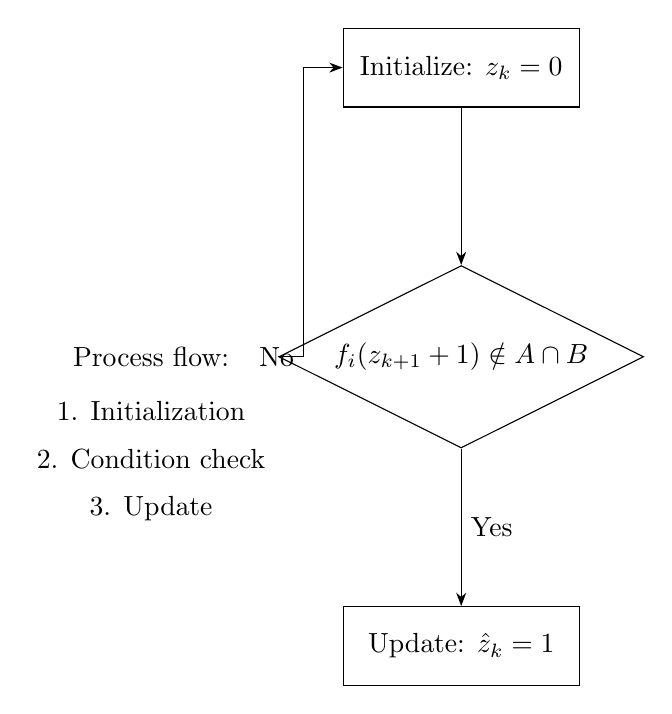
\begin{tikzpicture}[
    node distance=2cm,
    process/.style={rectangle, draw, minimum width=3cm, minimum height=1cm},
    condition/.style={diamond, draw, aspect=2, minimum width=2cm},
    arrow/.style={-Stealth}
]

% Nodes
\node (start) [process] {Initialize: $z_k = 0$};
\node (cond) [condition, below=of start] {$f_i(z_{k+1} + 1) \notin A \cap B$};
\node (result) [process, below=of cond] {Update: $\hat{z}_k = 1$};

% Arrows
\draw[arrow] (start) -- (cond);
\draw[arrow] (cond) -- node[right] {Yes} (result);
\draw[arrow] (cond) -- ++(-2,0) node[left] {No} |- (start.west);

% Annotations
\node[left=0.5cm of cond] (annot1) {Process flow:};
\node[below=0.2cm of annot1] {1. Initialization};
\node[below=0.8cm of annot1] {2. Condition check};
\node[below=1.4cm of annot1] {3. Update};

\end{tikzpicture}
\end{document}